\documentclass[border=10pt]{standalone}
\usepackage{tikz}\usepackage{amsmath}\usetikzlibrary{arrows.meta}
\begin{document}
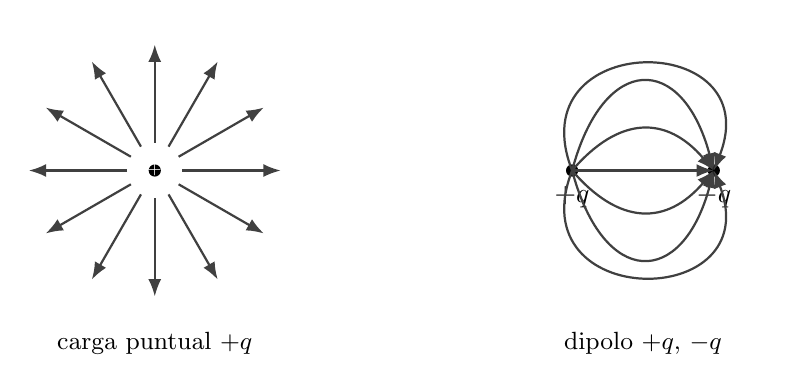
\begin{tikzpicture}[line width=0.8pt,>={Latex[length=2.2mm]}]
  % carga puntual positiva: lineas radiales salientes
  \fill (0,0) circle(2.2pt);
  \node at (0,0)[white]{\tiny$+$};
  \foreach \a in {0,30,...,330} \draw[->,black!75] (\a:0.35)--(\a:1.6);
  \node at (0,-2.2){\small carga puntual $+q$};
  % dipolo
  \begin{scope}[xshift=6.2cm]
    \fill (-0.9,0) circle(2.2pt) node[below=2pt]{$+q$};
    \fill (0.9,0) circle(2.2pt) node[below=2pt]{$-q$};
    \foreach \s in {1,-1}{
      \draw[->,black!75] (-0.9,0) .. controls (-0.3,\s*0.7) and (0.3,\s*0.7) .. (0.9,0);
      \draw[->,black!75] (-0.9,0) .. controls (-0.5,\s*1.5) and (0.5,\s*1.5) .. (0.9,0);
      \draw[->,black!75] (-0.9,0) .. controls (-1.6,\s*1.8) and (1.6,\s*1.8) .. (0.9,0);
    }
    \draw[->,black!75] (-0.9,0)--(0.9,0);
    \node at (0,-2.2){\small dipolo $+q,\,-q$};
  \end{scope}
\end{tikzpicture}
\end{document}
